\documentclass[11pt,a4paper]{article}
\usepackage[margin=2.25cm]{geometry}
\usepackage{booktabs}
\usepackage{amsmath}
\usepackage{siunitx}
\usepackage{hyperref}
\usepackage{xcolor}
\usepackage{datetime}
\usepackage{adjustbox}
\usepackage{float}
\newdateformat{monthyeardate}{\monthname[\THEMONTH] \THEYEAR}
\setlength{\tabcolsep}{4pt}

\title{When to Tune, When to Scale: Full FT vs.\ LoRA vs.\ Base Size Under Latency and Accuracy Constraints}
\author{Alberto Rodero\thanks{Equal contribution} \and Pablo Lobato\footnotemark[1]}
\date{September 2025}

\sisetup{
  round-mode=places,
  round-precision=3,
  table-number-alignment=center
}

\begin{document}
\maketitle

\section{Motivation \& Context}
Large Language Models (LLMs) are increasingly deployed under tight \textit{latency}, \textit{cost}, and \textit{governance} constraints. Relying solely on closed API models creates operational risks (variable token pricing, rate limits, model deprecations/renames, slower release cycles, and vendor lock-in), while on-prem or edge deployments demand predictable throughput and VRAM-aware footprints. In this context, teams face a practical choice: \emph{scale up} to a larger base model, or \emph{tune} a smaller one to the task.

\paragraph{Why these techniques.}
\textbf{Full fine-tuning} (NoPeft) offers maximal capacity to adapt behaviors but requires more compute and careful lifecycle management. \textbf{Parameter-Efficient Fine-Tuning} (PEFT), notably \textbf{LoRA}\cite{lora}, promises much lower VRAM and faster iteration by training small adapter matrices. However, open questions persist about the efficacy gap vs.\ full FT, the end-to-end \emph{latency/throughput} implications at inference, and how LoRA \emph{rank} impacts results in practice.

\paragraph{Why these models.}
We study \textbf{Qwen3-0.6B} and \textbf{Qwen3-1.7B}, two open-weight checkpoints from the same family. This pairing controls architectural confounds, represents a realistic size jump (0.6B $\rightarrow$ 1.7B) seen in production trade-offs, fits commodity GPUs, and is widely used in on-prem/edge scenarios. It also reflects a common decision boundary: \emph{``Should we tune the small model we can host cheaply, or trade latency to a larger untuned model?''}

\paragraph{Why now.}
As API prices and policies fluctuate and new frontier releases arrive on slower cadences, organizations increasingly need \textit{controllable}, \textit{auditable}, and \textit{cost-stable} stacks. Evaluating when to \emph{tune} vs.\ when to \emph{scale}---and whether PEFT is ``good enough'' under real latency budgets---is therefore critical.

\paragraph{Our aim.}
We provide actionable guidance on accuracy--latency trade-offs across \textbf{full FT} vs.\ \textbf{LoRA (various ranks)} vs.\ \textbf{base size}, using three complementary task families (ARC, OpenMath, SQuAD v2). We also surface the impact of uncontrolled \emph{reasoning} behavior (a realistic deployment confound we later discuss in Sec.~\ref{sec:setup}) to inform \textbf{production decisions}.

\paragraph{Key questions.}
\begin{itemize}
  \item \textbf{Q1:} Is fine-tuning worth it in efficacy and efficiency?
  \item \textbf{Q2:} How does a fine-tuned 0.6B compare to a larger 1.7B base?
  \item \textbf{Q3:} If VRAM is abundant, is LoRA still worth using?
  \item \textbf{Q4:} Does LoRA rank materially affect outcomes?
  \item \textbf{Q5:} Partial vs.\ full tuning: LoRA vs.\ NoPeft?
  \item \textbf{Q6:} Cross-task transfer effects?
  \item \textbf{Q7:} If VRAM forces LoRA, is fine-tuning still worth it?
\end{itemize}

\section{Experimental Setup}
\label{sec:setup}
\paragraph{Models.}
We compare \textbf{Qwen3-0.6B} under two tuning regimes—\textbf{full fine-tuning (NoPeft)} and \textbf{LoRA} with ranks $r\in\{32,64,256,512,1024\}$—against \textbf{Qwen3-0.6B base} and a larger \textbf{Qwen3-1.7B base}. We \textbf{do not use quantization} in any reported run; this isolates the effects of the fine-tuning method, rank, and configuration from quantization-related confounds.

\paragraph{Datasets.}
We evaluate on three task families:
\begin{itemize}
  \item \textbf{ARC\cite{arc} (AI2 ARC, 4-way MCQ).} Multiple-choice science questions; we compute macro-F1 across options A/B/C/D.
  \item \textbf{OpenMathInstruct-2\cite{openmath} (numeric).} Free-form numeric answers; we report average absolute difference (lower is better).
  \item \textbf{SQuAD v2\cite{squad} (extractive QA).} Span extraction with unanswerable cases; we report F1 and EM in the evaluator.
\end{itemize}

\paragraph{Frameworks.}
We use \textbf{HuggingFace Transformers}\cite{huggingfaceTransformers} (\texttt{AutoModelForCausalLM}, \texttt{AutoTokenizer}), \textbf{TRL} (\texttt{SFTTrainer}, \texttt{SFTConfig}) for supervised fine-tuning, and \textbf{PEFT} (\texttt{LoraConfig}, \texttt{get\_peft\_model}). Execution is PyTorch (\texttt{bfloat16} on CUDA when available).

\paragraph{Supervised fine-tuning (SFT).}
Each dataset is preprocessed into a simple chat-style format (single user turn with optional context; single assistant completion). Tokenizer uses EOS as pad if unset and a minimal chat template. Global training hyperparameters:
\begin{itemize}
  \item \textbf{Optimizer/schedule (via TRL defaults):} \texttt{learning\_rate $\;1\!\times\!10^{-5}$}, \texttt{warmup\_ratio=0.06}, \texttt{weight\_decay=0.0}, \texttt{max\_grad\_norm=1.0}.
  \item \textbf{Batching:} \texttt{per\_device\_train\_batch\_size=1}, \texttt{gradient\_accumulation\_steps=8} (effective batch $=8$), \texttt{num\_train\_epochs=1}.
  \item \textbf{Sequence length:} \texttt{max\_length=1024}, \texttt{packing=False}, \texttt{assistant\_only\_loss=False}.
  \item \textbf{Memory:} \texttt{gradient\_checkpointing=True}.
\end{itemize}
\textbf{NoPeft} updates all weights. \textbf{LoRA} targets attention projections \{\texttt{q\_proj}, \texttt{k\_proj}, \texttt{v\_proj}, \texttt{o\_proj}\} with \texttt{lora\_alpha=16}, \texttt{lora\_dropout=0.1}; ranks $r$ as above. After SFT, LoRA adapters are merged for evaluation.

\paragraph{Evaluation protocol.}
We run a deterministic, non-sampling decode (\texttt{do\_sample=False}; \texttt{temperature=None}, \texttt{top\_p=None}, \texttt{top\_k=None}; \texttt{max\_new\_tokens=1000}). Each dataset is associated with a concise \emph{system prompt} that standardizes the expected output format using \verb|\boxed{...}| (e.g., \verb|\boxed{C}| for ARC; exact span for SQuAD; numeric for OpenMath). Latency is measured as wall-clock time of a full \texttt{generate()} call per sample. We also record output token counts via the tokenizer.

\paragraph{Metrics.}
\begin{itemize}
  \item \textbf{ARC:} macro-F1 across A/B/C/D from a 4-class confusion matrix; we additionally track accuracy.
  \item \textbf{OpenMathInstruct-2:} average absolute difference between predicted and gold numeric answers (tolerance $10^{-4}$); we also report accuracy (within tolerance).
  \item \textbf{SQuAD v2:} EM and F1 with standard normalization (lowercasing, punctuation/article removal), plus AvNA and No-Answer accuracy; we report F1 in the main table.
  \item \textbf{Latency:} per-sample seconds and aggregates (mean/median/std).
\end{itemize}

\paragraph{Runtime, decoding \& confounds.}
We place models via \texttt{device\_map} (GPU when available) and use \texttt{bfloat16} on CUDA. Decoding is deterministic (no sampling). \emph{Reasoning-like behavior is intentionally left unlocked at inference time}: we do not enforce a specific “reasoning mode” so that differences reflect the \textbf{effect of fine-tuning itself} on \emph{when} the model chooses to reason and \emph{how much} it reasons (versus responding directly). This design helps isolate tuning-induced shifts in reasoning propensity, but it also introduces variance in latency and accuracy. Additional confounds: single-seed/shot artifacts may exist; measured latency depends on this pipeline/hardware; and we did not run calibration/temperature sweeps.


\paragraph{Scope.}
This study focuses strictly on \textbf{full SFT (NoPeft)} vs.\ \textbf{LoRA}. We do not report quantized-training variants (e.g., QLoRA) or alternative adapters (DoRA/VeRA), nor do we sweep decoding temperatures or instruction-following prompts. These choices are deliberate to isolate the \emph{tuning method vs.\ base size} question.

\vspace{370pt}
\section{Full Results Table}
\label{sec:fulltable}

\noindent\textit{Notes:} ``Math AbsDiff\,$\downarrow$'' is lower=better. Latencies are seconds.

\begin{table}[H]
\centering
\caption{Full results across tasks. Lower is better for Math AbsDiff. Latency in seconds. Best \emph{efficacy} and \emph{efficiency} (latency) within each training block are \textbf{bolded}.}
\label{tab:full}
\footnotesize
\begin{adjustbox}{max width=\textwidth}
\begin{tabular}{lllrrrrrr}
\toprule
 & & & \multicolumn{2}{c}{\textbf{ARC}} & \multicolumn{2}{c}{\textbf{OpenMath}} & \multicolumn{2}{c}{\textbf{SQuAD v2}} \\
\cmidrule(lr){4-5}\cmidrule(lr){6-7}\cmidrule(lr){8-9}
\textbf{Base} & \textbf{PEFT} & \textbf{$r$} & \textbf{F1 $\uparrow$} & \textbf{Lat $\downarrow$} & \textbf{AbsDiff $\downarrow$} & \textbf{Lat $\downarrow$} & \textbf{F1 $\uparrow$} & \textbf{Lat $\downarrow$} \\
\midrule
\multicolumn{9}{l}{\textit{Trained on ARC}} \\
Qwen3-0.6B & LoRA   & 1024 & 0.4921 & 0.1557 & \textbf{22{,}871} & 0.4374 & 8.59 & \textbf{0.1939} \\
Qwen3-0.6B & LoRA   & 512  & 0.4861 & 0.1570 & \textbf{22{,}871} & 0.4312 & 8.59 & 0.1955 \\
Qwen3-0.6B & LoRA   & 256  & 0.4921 & 0.1549 & \textbf{22{,}871} & 0.4191 & 8.59 & 0.1948 \\
Qwen3-0.6B & LoRA   & 64   & \textbf{0.4937} & 0.1601 & \textbf{22{,}871} & \textbf{0.1811} & 8.09 & 0.1952 \\
Qwen3-0.6B & LoRA   & 32   & 0.4880 & 0.1595 & \textbf{22{,}871} & 0.4439 & 8.59 & 0.1958 \\
Qwen3-0.6B & NoPeft & --   & 0.4905 & \textbf{0.0803} & 23{,}108 & 0.2137 & \textbf{18.89} & 0.2003 \\
\midrule
\multicolumn{9}{l}{\textit{Trained on OpenMath}} \\
Qwen3-0.6B & LoRA   & 1024 & 0.4990 & 0.9257 & 23{,}919 & 1.5384 & \textbf{8.48} & 0.2091 \\
Qwen3-0.6B & LoRA   & 256  & 0.5031 & 0.8982 & 23{,}655 & 1.5016 & \textbf{8.48} & \textbf{0.1934} \\
Qwen3-0.6B & LoRA   & 32   & 0.5095 & 0.8702 & 23{,}919 & 1.5776 & \textbf{8.48} & 0.1963 \\
Qwen3-0.6B & NoPeft & --   & \textbf{0.5171} & \textbf{0.0605} & \textbf{16{,}540} & \textbf{0.0482} & 7.40 & 0.2439 \\
\midrule
\multicolumn{9}{l}{\textit{Trained on SQuAD v2}} \\
Qwen3-0.6B & LoRA   & 1024 & \textbf{0.5024} & 0.3178 & 23{,}647 & 2.1285 & 9.59 & 0.1951 \\
Qwen3-0.6B & LoRA   & 256  & \textbf{0.5024} & 0.3116 & 23{,}647 & 2.0291 & 9.59 & \textbf{0.1908} \\
Qwen3-0.6B & LoRA   & 32   & \textbf{0.5024} & 0.3095 & 23{,}523 & 1.9676 & 9.59 & 0.1950 \\
Qwen3-0.6B & NoPeft & --   & 0.4542 & \textbf{0.1903} & \textbf{22{,}997} & \textbf{0.2203} & \textbf{27.95} & 0.2202 \\
\midrule
\multicolumn{9}{l}{\textit{Base models (no fine-tuning)}} \\
Qwen3-0.6B & Base   & --   & 0.4932 & \textbf{1.1397} & 24{,}834 & \textbf{6.0139} & 10.07 & \textbf{0.2274} \\
Qwen3-1.7B & Base   & --   & \textbf{0.7986} & 3.4025 & \textbf{742} & 12.5197 & \textbf{30.36} & 0.2837 \\
\bottomrule
\end{tabular}
\end{adjustbox}
\end{table}

\section{Results by Question \& Interpretation}

\subsection*{Q1. Is fine-tuning worth it (efficacy \& efficiency)?}
\textbf{Yes, when aligned to the target task, fine-tuning yields large quality gains and often lower latency.} 
\begin{itemize}
  \item \textbf{OpenMath SFT (NoPeft)}: Math abs diff improves by \textbf{33.4\%} vs 0.6B\_base; ARC macro-F1 rises \textbf{+4.8\%}; SQuAD F1 drops \textbf{--26.5\%}. Latency massively drops on ARC (\textbf{--94.7\%}) and Math (\textbf{--99.2\%}), small increase on SQuAD (\textbf{+7.3\%}).
  \item \textbf{SQuAD SFT (NoPeft)}: SQuAD F1 jumps \textbf{+177.6\%}; ARC macro-F1 dips \textbf{--7.9\%}; Math improves mildly (\textbf{+7.4\%} abs-diff reduction). Latency generally improves (ARC \textbf{--83.3\%}, Math \textbf{--96.3\%}, SQuAD \textbf{--3.2\%}).
\end{itemize}
\textit{Why?} Full-task alignment amplifies the relevant capabilities and stabilizes decoding behavior; our pipeline also appears to run tuned checkpoints more efficiently.

\subsection*{Q2. Fine-tuned 0.6B vs.\ larger 1.7B base?}
\textbf{The 1.7B base dominates on quality but is slower.} 
ARC macro-F1 +61.9\%, Math abs diff $\sim$97\% better, and SQuAD F1 +201.5\% vs 0.6B\_base. Latency worsens markedly (ARC +198.5\%, Math +108.2\%, SQuAD +24.8\%). 
\textbf{If latency/throughput matters, 0.6B + targeted SFT is the speed/price sweet spot.}

\subsection*{Q3. If VRAM is not a problem, should we still use LoRA?}
\textbf{No. Prefer full fine-tuning.} In these runs, \textbf{NoPeft is both more accurate and often faster} than LoRA (Table~\ref{tab:lora_vs_nopeft}). The only place where NoPeft is slightly slower is SQuAD (+0.029\,s), but it delivers a \textbf{+18.36} absolute F1 jump over the best LoRA.

\begin{table}[htbp]
\centering
\caption{Best LoRA vs.\ NoPeft by task. For OpenMath, lower is better (AbsDiff$\downarrow$). Latency in seconds. Within each task, best \emph{score} and best \emph{latency} are \textbf{bolded}.}
\label{tab:lora_vs_nopeft}
\footnotesize
\begin{adjustbox}{max width=\textwidth}
\begin{tabular}{llrccrr}
\toprule
 & & & \multicolumn{2}{c}{\textbf{LoRA (best)}} & \multicolumn{2}{c}{\textbf{NoPeft (best)}} \\
\cmidrule(lr){4-5}\cmidrule(lr){6-7}
\textbf{Task} & \textbf{Base} & \textbf{LoRA $r$} & \textbf{Score} & \textbf{Lat $\downarrow$} & \textbf{Score} & \textbf{Lat $\downarrow$} \\
\midrule
ARC (F1 $\uparrow$) & Qwen3-0.6B & 64   & \textbf{0.4937} & 0.1601 & 0.4905 & \textbf{0.0803} \\
OpenMath (AbsDiff $\downarrow$) & Qwen3-0.6B & 256  & 23{,}655 & 1.5016 & \textbf{16{,}540} & \textbf{0.0482} \\
SQuAD v2 (F1 $\uparrow$) & Qwen3-0.6B & 1024 & 9.59 & \textbf{0.1951} & \textbf{27.95} & 0.2202 \\
\bottomrule
\end{tabular}
\end{adjustbox}
\end{table}


\subsection*{Q4. Does LoRA rank matter?}
\textbf{Little to no consistent improvement from using higher ranks.}
Correlation between rank and score (LoRA-only subsets): \textbf{ARC F1:} $\rho\!=\!0.021$; \textbf{OpenMath abs diff:} $\rho\!=\!0.301$ (higher rank slightly worse); \textbf{SQuAD F1:} constant across ranks (no signal). Rank vs.\ latency shows weak-to-moderate links (e.g., ARC $\rho\!=\!-0.646$ hints at slightly lower latency at higher ranks), but the absolute differences are tiny.
\begin{table}[h!]
\centering
\caption{Correlation between LoRA rank and performance/latency (LoRA-only).}
\label{tab:correlations}
{\small
\begin{tabular}{lrr}
\toprule
Task & Corr(rank, score) & Corr(rank, latency) \\
\midrule
ARC (F1) & 0.021 & -0.646 \\
OpenMath (AbsDiff$\downarrow$) & 0.301 & -0.233 \\
SQuAD (F1) & N/A & 0.321 \\
\bottomrule
\end{tabular}
}
\end{table}

\textit{Why might rank not matter much?} With limited data or strongly structured tasks, the low-rank subspace often captures the critical adaptations; beyond a point, extra capacity (higher rank) faces diminishing returns and optimization noise. Also, our decoding and “reasoning” variability likely masks small rank effects.

\subsection*{Q5. LoRA (partial) vs.\ NoPeft (full) training?}
\textbf{Full fine-tuning wins decisively.}
\begin{itemize}
  \item \textbf{OpenMath:} NoPeft improves error by \textbf{7{,}115} absolute over the best LoRA and is \textbf{$\sim$1.45\,s} faster.
  \item \textbf{SQuAD v2:} NoPeft improves F1 by \textbf{+18.36} with only a \textbf{+0.029\,s} latency penalty.
  \item \textbf{ARC:} NoPeft is \textbf{$\sim$2$\times$ faster} than the best LoRA, with essentially tied F1.
\end{itemize}

\subsection*{Q6. Cross-task transfer?}

\paragraph{Catastrophic forgetting (CF).}
CF is the degradation of previously acquired capabilities when fine-tuning on a new task. It is distinct from benign \emph{negative transfer} (where a skill conflicts but is still partly retained). In our single-task SFT runs, we observe patterns consistent with CF on some capabilities:

\begin{itemize}
  \item \textbf{OpenMath SFT (NoPeft)} $\rightarrow$ \textit{SQuAD:} \textbf{--26.5\%} F1 indicates a substantial loss of extractive-span behavior, beyond mild interference. In contrast, \textit{ARC} improves \textbf{+4.8\%}, suggesting numeric SFT does not erase MCQ.
  \item \textbf{SQuAD SFT (NoPeft)} $\rightarrow$ \textit{ARC:} \textbf{--7.9\%} (moderate), while \textit{Math} slightly improves \textbf{+7.4\%}. This looks more like cross-task interference than severe CF.
  \item \textbf{ARC SFT (NoPeft)} $\rightarrow$ \textit{SQuAD:} \textbf{+87.6\%} (surprisingly positive), and \textit{Math:} \textbf{+7.0\%}; \textit{ARC} self-performance is \textbf{--0.5\%} (negligible). Here ARC seems to prime general reading/selection skills that transfer to extractive QA.
\end{itemize}

\paragraph{PEFT vs.\ full FT.}
LoRA variants show \emph{smaller cross-task shifts} than NoPeft in several cases (e.g., OpenMath~SFT $\rightarrow$ SQuAD: LoRA $\approx 8.48$ F1 vs.\ NoPeft $7.40$; ARC~SFT $\rightarrow$ SQuAD: LoRA $\approx 8\!-\!8.59$ vs.\ NoPeft $18.89$). This suggests LoRA \emph{can} mitigate forgetting by restricting updates, but it may also \emph{limit positive transfer} when full FT would have helped. In short: \textbf{NoPeft magnifies both upside and downside}; LoRA dampens both.

\paragraph{Interpretation.}
Extractive QA (SQuAD) and numeric reasoning (OpenMath) compete for representational capacity in different subskills (span extraction vs.\ procedural computation). Tuning toward one can suppress the other. ARC SFT (full) appears to reinforce token-level selection and short-answer discipline, which transfers to SQuAD.

\paragraph{Takeaway.}
In our setting, \textbf{OpenMath$\rightarrow$SQuAD degradation under NoPeft} is the clearest CF signal; \textbf{SQuAD$\rightarrow$ARC} looks like moderate interference; and \textbf{ARC$\rightarrow$SQuAD} shows strong positive transfer. Choosing \emph{when to use full FT vs.\ LoRA} is therefore also a choice about \emph{risk/reward on forgetting vs.\ transfer}.

\subsection*{Q7. If VRAM forces LoRA, is it still worth it?}
\textbf{Yes, but temper expectations.} 
OpenMath LoRA-256 reduces error by \textbf{4.8\%} vs 0.6B\_base (useful), but SQuAD LoRA variants lose \textbf{$\sim$4.8\%} F1 vs 0.6B\_base, and ARC LoRA gains are marginal (\textbf{+0.1\%}). 
\textbf{Recommendation:} When constrained, \textbf{LoRA~$\approx$~256} is a good default; otherwise prefer NoPeft.

\begin{figure}[H]
    \centering
    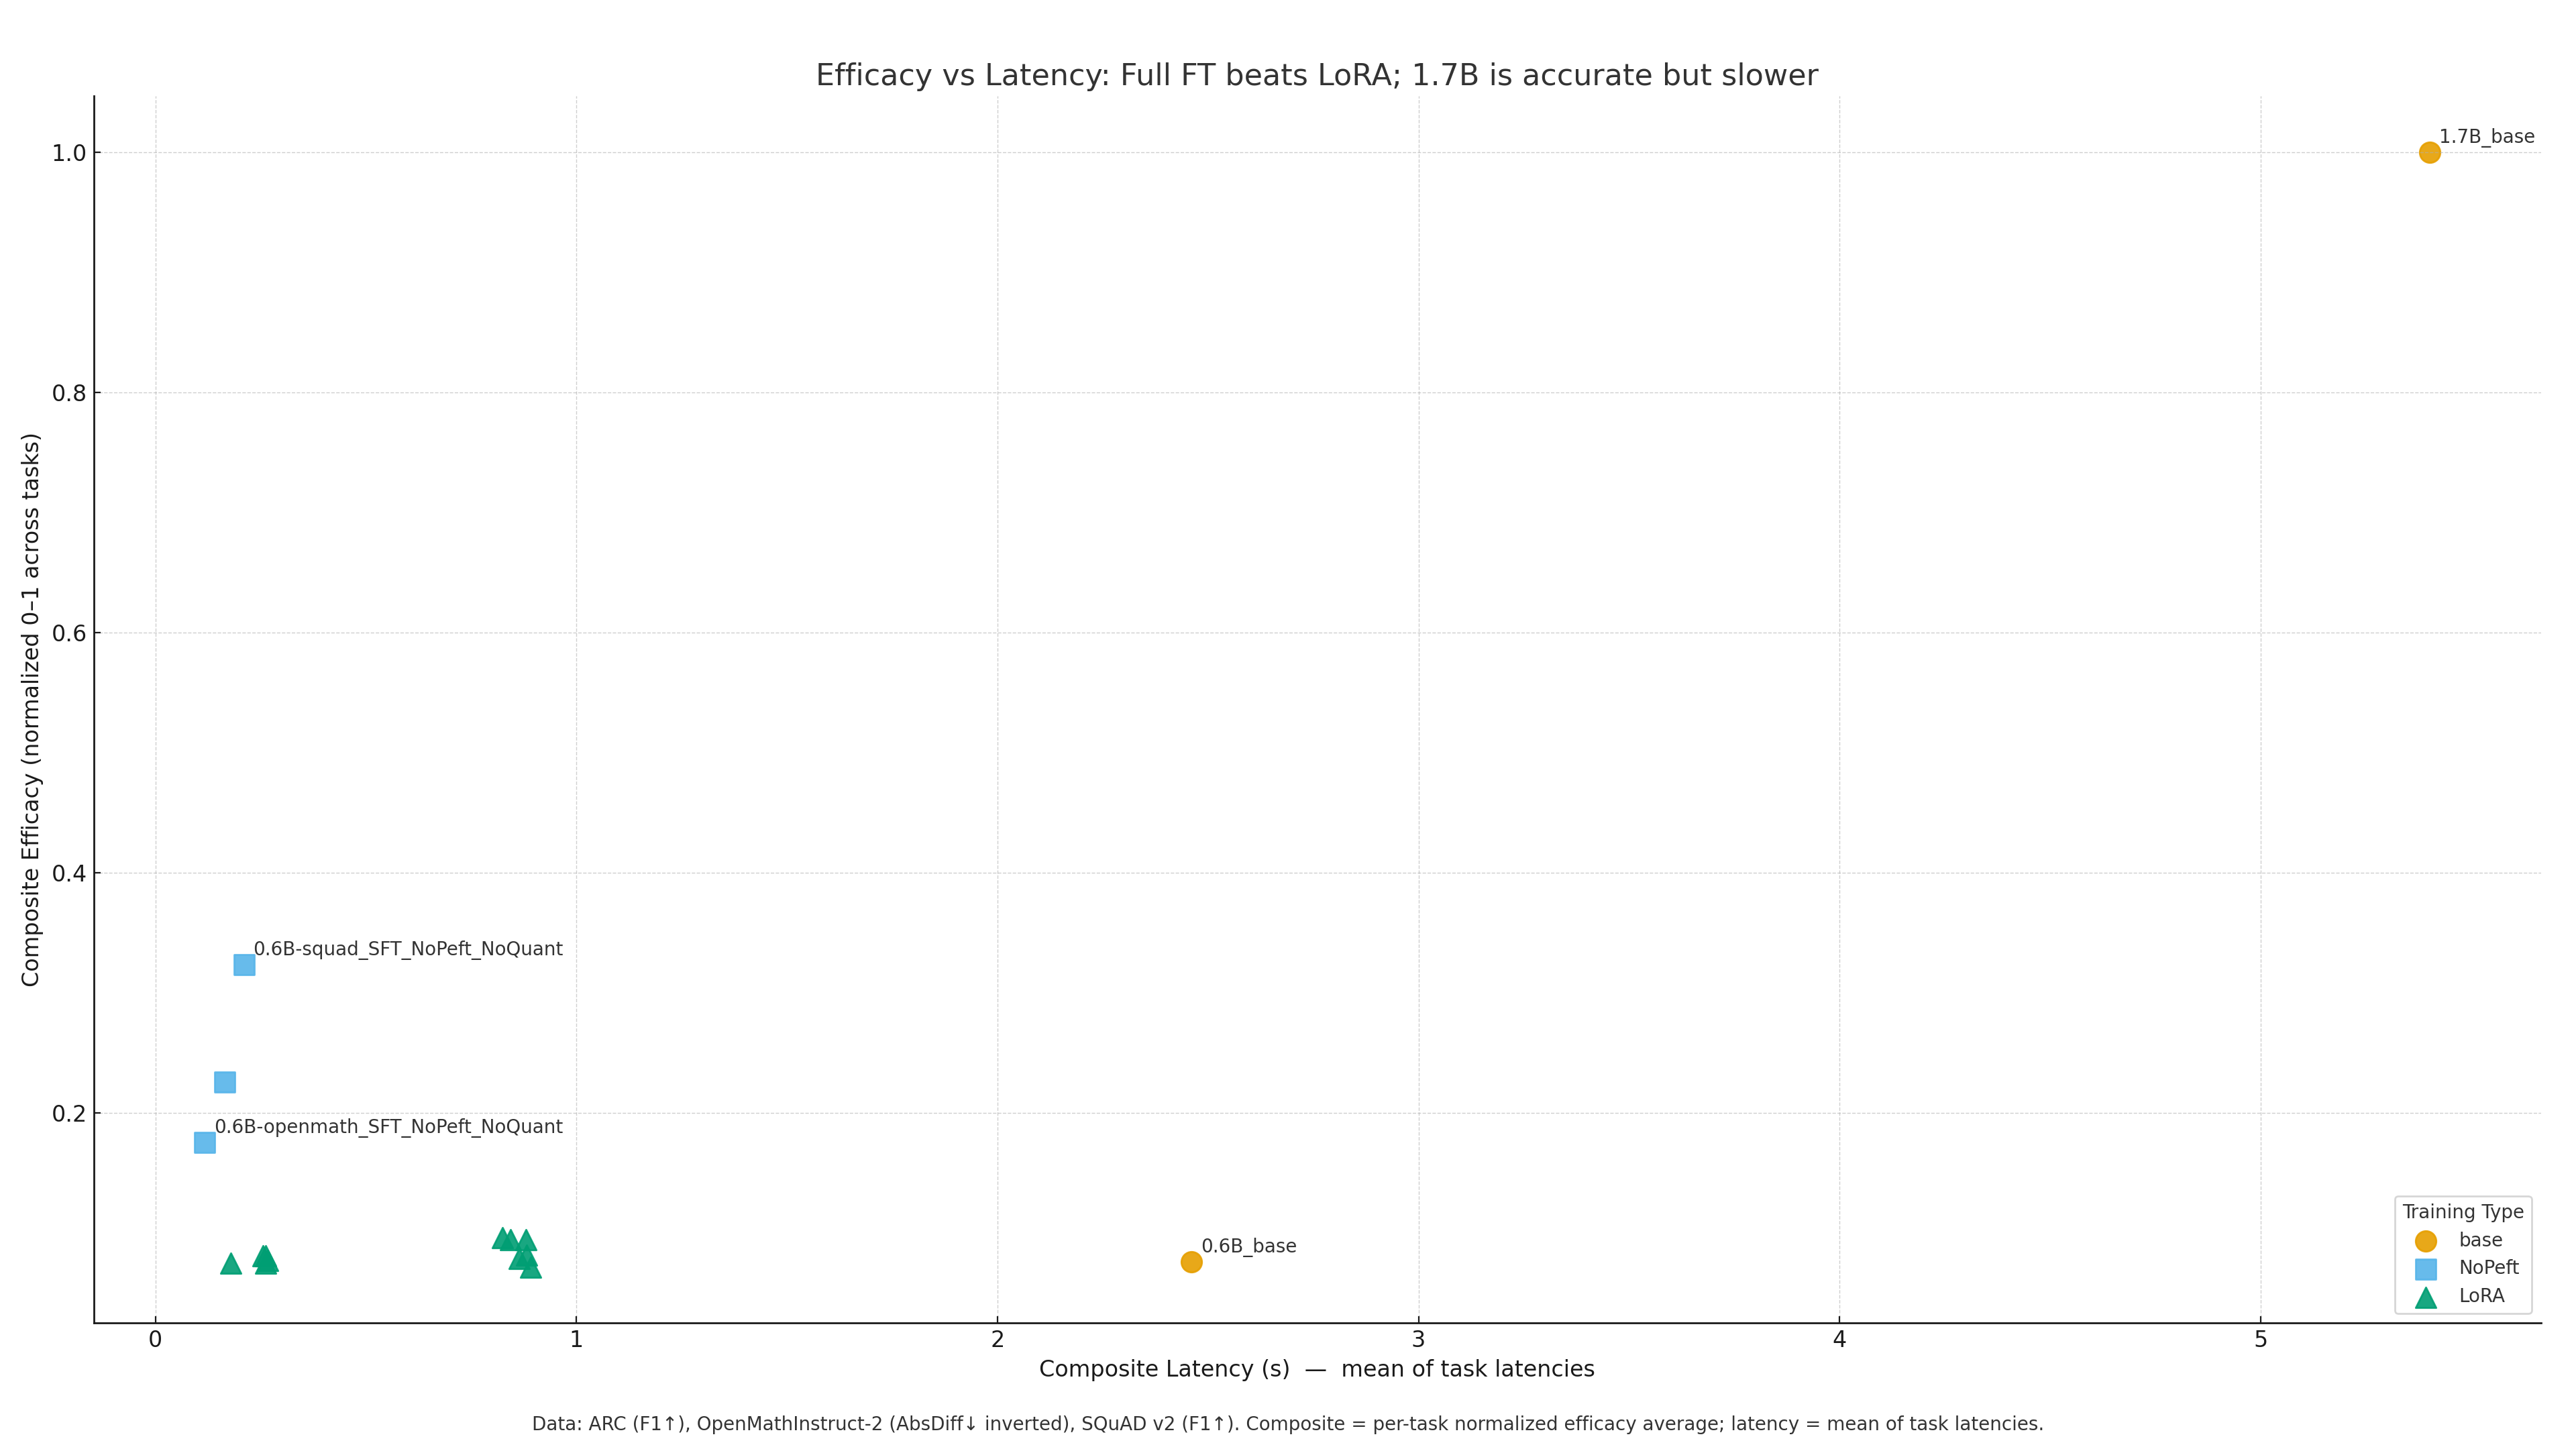
\includegraphics[width=1\linewidth]{01_Finetuning_ModelSize_LoraR.png}
    \caption{Efficacy vs Latency}
    \label{fig:placeholder}
\end{figure}

\section{Conclusions \& Takeaways}
\textit{We summarize two complementary views: (i) technical takeaways that guide modeling choices, and (ii) practical conclusions for solution design.}

\begin{itemize}
  \item \textbf{(1) Full fine-tuning beats LoRA on both accuracy and, in these runs, speed.}
  
  \item \textbf{(2) A larger base model is best on accuracy but slower; 0.6B+SFT is the speed/value sweet spot.}
  
  \item \textbf{(3) LoRA rank has weak, non-predictable effects; use $\sim$256 by default when constrained.}

  \item \textbf{(4) Practical decision rule.} \emph{Start small and tune.} If the tuned 0.6B misses the quality bar, try task-specific SFT refinements (data curation, longer context, decoding hygiene). \emph{Only then} consider scaling to 1.7B if accuracy remains the blocker and latency/cost allow.

  \item \textbf{(5) When to prefer LoRA.} Use LoRA if VRAM is tight, you need \emph{multiple domain adapters} with hot-swapping, or you want safer edits that reduce catastrophic forgetting. Keep $r\!\approx\!256$ as a strong default; raise $r$ only with evidence.

  \item \textbf{(6) Forgetting vs.\ transfer.} Full SFT amplifies both \emph{upside} (positive transfer) and \emph{downside} (catastrophic forgetting). If cross-task robustness matters, use multi-task/rehearsal SFT, per-task adapters with routing/fusion, or light regularization/distillation.

  \item \textbf{(7) Cost/ops note.} Tuned small models reduce serving cost and throughput variance; larger bases raise accuracy ceilings but increase latency and hardware requirements. Choose based on the product’s \emph{primary constraint} (SLO latency vs.\ target quality).
\end{itemize}

\subsection*{Practical conclusions}
\textit{What do these results mean at a high level?} \textbf{Context-anchored tasks (e.g., RAG/extractive QA) are easier to lift with SFT}, because fine-tuning efficiently aligns span selection, formatting, and instruction adherence when relevant context is provided. \textbf{Procedural/logic tasks (e.g., math) benefit more from full FT with richer supervision or from scaling the base model (often with tool use)}, as they require deeper representational shifts. In practice, a \emph{small fine-tuned model} can often meet quality targets for RAG-style workloads while lowering latency and cost versus a larger hosted API; reserve \textbf{LoRA} for VRAM-constrained setups or rapid domain switching.

\begin{thebibliography}{99}

\bibitem{lora} Edward J. Hu, Yelong Shen, Phillip Wallis, Zeyuan Allen-Zhu, Yuanzhi Li, Shean Wang, Lu Wang and Weizhu Chen; ``LoRA: Low-Rank Adaptation of Large Language Models'', {\it arXiv}, 2021.

\bibitem{arc} Ai2\_arc. Disponible en {\it https://huggingface.co/datasets/allenai/ai2\_arc}. Consultado el 1 de septiembre de 2025.
\bibitem{openmath} Open Math Instruct-2. Disponible en {\it https://huggingface.co/datasets/nvidia/OpenMathInstruct-2}. Consultado el 1 de septiembre de 2025.
\bibitem{squad} Squad\_v2. Disponible en {\it https://huggingface.co/datasets/rajpurkar/squad\_v2}. Consultado el 1 de septiembre de 2025.
\bibitem{huggingfaceTransformers} Hugging Face Transformers. Disponible en {\it https://huggingface.co/docs/transformers/en/index}. Consultado el 4 de septiembre de 2025.

\end{thebibliography}

\end{document}
